\chapter{Serverless architecture for web applications}

\section{Intro}

\subsection{Motivation}

\begin{enumerate}
    \item serverless most frequently used for web apps (summary of research papers)
\end{enumerate}

\subsection{Research questions}

\begin{enumerate}
    \item Is serverless paradigm suitable for building web applications?
    \item Server tier - How the serveless processing model can be utilised to perform web application business logic?
    \item Data tier - How the storage systems are leveraged in the serverless paradigm?
    \item Client tier
\end{enumerate}

\subsection{Research approach}

\begin{enumerate}
    \item Why AWS?
    \item How the research looks like? 2 - 3 examples / case studies + minor architecture implementations
\end{enumerate}

\section{Serverless suitability for web applications}

\subsection{Web app requirements}

considering the web application requirements mentioned in chapter \ref{section:web-apps-requirements}

\subsection*{Performance and Scalability}

% web applications
- performance from the user point of view - how fast the requests are fulfilled
- performance fro the system point of view - many users performing actions at the time - application need to perform properly when the load is increased - system should scale to meet the demand

- in case of serverless - horizontal scaling managed by the platform - allocating new resources absed on the events comming to the system, due to stateless architecture
- some serverless, stateful storage components designed to work at scale - S3, DynamoDB
- on the other hand - unpredictable performance, colds starts
- by default lambda concurrency is limitted - can be increased when discussed with the provider

---

\subsection*{Reliability}

% web applications
system continue correctly event when failure in some other part of application, resilience and fault tolerance, preventin app from stopping once error occurs

- some of the serverless components are designed for failures - DLQ, Lambda destination - it needs to be handled by the developer to filter out and store all the failures
- operating across multiple regions, availability zones - these are not connected with each other, even when one fail, the other should work, the architecture can operate on both of them
- embracing automation to ensure good quality of service - automation tests running before the deployment, stress/load testing - due to the fact that serverless paradigm requires to run the app on the host platform it is worth it to automate the processes
- logging, monitoring, CloudWatch alarms, ensuring proper level of observability is required

---

\subsection*{Security and Compliance}

% web applications
- larger and not fully researched area, some of the articles considering security gaps in the cloud providers platforms - bug bounty programs
- by default - access denied
- user authentication mechanism + proper configuration should prevent from accessing the resources without permissions (similar to traditional web apps, but in that case we're utilising most frequently the mechanism provided by the cloud vendor - which is not that trivial, which is thoughtfully tested, instead of the one developed by ourselves, which can include some security gaps)
- fine grained IAM (Identity and Access Management) rules - FaaS should have no more than only the required permissions to other services - it could be difficult for larger applications more fine grained functions/resources

---

\subsection*{Maintainability}

% web applications
- no need to maintain the servers, no operational work with configuring them

developers perspective
- initially it reduces the amount of work developers neeed to do - utilising serverless components offered by the platform, new development opportunities - shorter lead time, greater agility
- maintainability of the larger applications can be also not trivial, looks different than the traditional applications - is there any research measing maintainability of the serveless aplication in the long run?

operational perspective
- no need to manage servers, handle scaling of the services
- monitoring, deployment, configuration management - could be more complex, without the knowledge of the platform

---

% \subsubsection*{Reduced development and operational cost}
% - serverless is another step in infrastructure management outsourcing, cloud platform is responsible for provisioning resources and executing it, responsibility for managing the servers, databases transfered to the cloud provider
% - less work related with managing the serverless solution 
%     - labour cost related with management and operational aspects
%     - development - using BaaS component replacing the application 

\subsection{Serverless suitability}

\begin{enumerate}
    \item reference to the use cases - application backend, event-driven data processing, real-time data stream
    \item (Adzic) Yubl \& MindMup - occasional, spiky traffic
    \item (Leveraging serverless cloud computing architectures) Types of workloads are suitable for serverless - irregular traffic, low traffic, workload parallelisation
    \item articles comparing serverless to microservices / monolith in case of performance
    \item examples from Berkeley - rethinking the processing - hybrid solutions with VMs when need to keep the state, use FaaS for parallelisation
    \item cost as important factor to consider
\end{enumerate}

\section{Example implementations}

\begin{figure}[h]
    \centering
    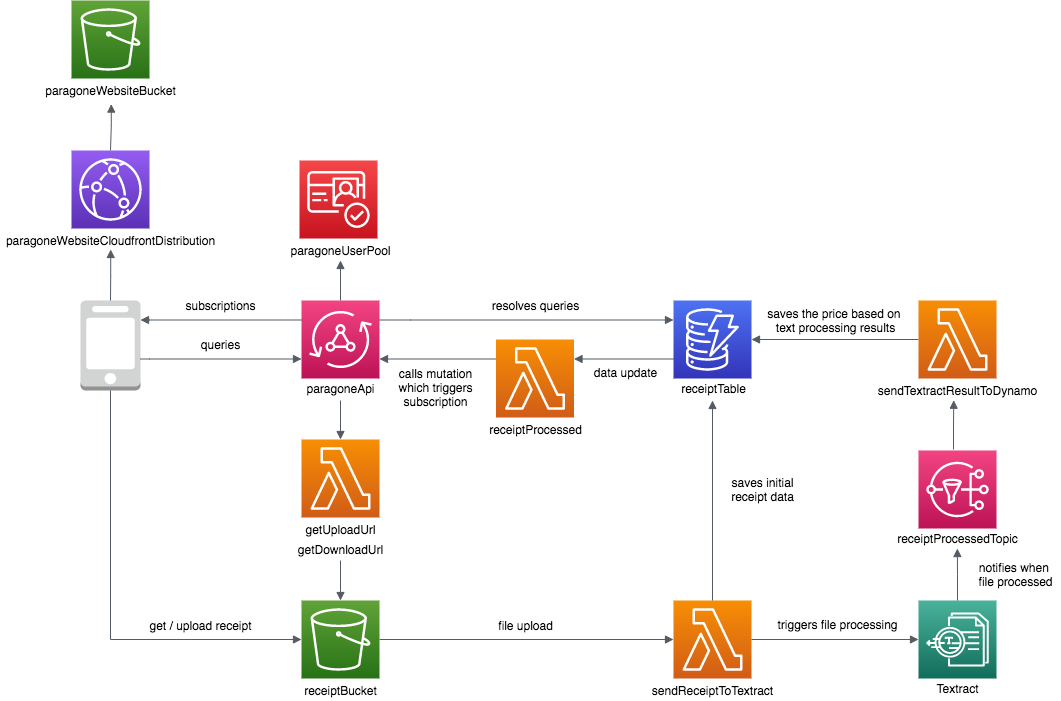
\includegraphics[width=1\textwidth]{assets/04-serverless-for-web-apps/paragoneArchitecture.png}
    \caption{Architecture of receipt processing web application}
    \label{fig:paragone-web-app}
\end{figure}

\begin{enumerate}
    \item small web app - processing receipts/invoices
    \item API performance comparison - containters / API Gateway + lambda + db / API Gateway directly to db
    \item parallelisation of processing - examples of video transcoding - AWS Step Function (compiling latex file to interactive presentation + orchestration) - performance / cost optimisation
    \item event-driven game / collaboration tool - is serverless feasible, compared to the application using containers (AppSync / websockets, persisting data in DynamoDB - what's the latency/cost)
    % https://serialized.net/2020/09/multiplayer/
    % https://serialized.net/2021/03/serverless_gaming_limits/
    % https://aws.amazon.com/blogs/compute/building-a-serverless-multiplayer-game-that-scales/
\end{enumerate}

Berkeley research papers example
    
https://aws.amazon.com/lambda/resources/reference-architectures/

\section{Server Tier}

\subsection{Serverless processing model / compared to microservices / event-driven}

% serverless vs microservices, serverless vs event-driven ~ event sourcing - similarities and differences

reference to articles comparing serverless / microservices / monolith for Web App API

\subsection{Web application workload types for serverless}

% event driven system - paragone, workload parallelisation - latex?, push based approach, pull based for workers when data is batched

synchronous - function needs to return smth and we're waiting till the services returns the data

asynchronous - calling services and finishing execution - smth other calls another lambda - SNS for pub/sub, SQS for batching - event stream triggering new services one after the other

function composition problems - StepFunction

fanout - utilising parallelisation - serverless benefits

% https://www.usenix.org/system/files/conference/hotcloud18/hotcloud18-paper-hong.pdf
% https://www.researchgate.net/profile/Davide-Taibi/publication/340121613_Patterns_for_Serverless_Functions_Function-as-a-Service_A_Multivocal_Literature_Review/links/5e79f9fb92851c3091392bd4/Patterns-for-Serverless-Functions-Function-as-a-Service-A-Multivocal-Literature-Review.pdf
% https://aws.amazon.com/lambda/resources/reference-architectures/

\subsection{Serverless function optimisation}

internals

composition - StepFunction

using with other services - push/pull/stream models - SNS / SQS / DynamoDB

CPU bound is feasible, I/O not

optimising cold starts

patterns

\section{Data Tier}

\subsection{Issues when integrating traditional databases with serverless}

\subsection{Serverless databases}

DynamoDB - modeling for cost optimisation, increase performance, single table design

Aurora

S3

how they work? streams, handling reusing connections, RDS proxy

\section{Client Tier}

\subsection{Client communication patterns with serverless architecture}

APIGateway - REST + websockets

AppSync - GraphQL - data aggregation from different resources

gatekeeper - authentication

direct resolvers to particular services with/without the lambda, pipeline resolvers (nested nodes in graph) - overhead comparison

calling the services from the client - presigned URLs / using client libs to have access to resources

\subsection{Serverless push based approach}

request - response

push to pull pattern

GraphQL subscriptions triggered by mutation

\subsection{Hosting web clients}

hosting static files

server side rendering

\section{Desing patterns and best practices}
